\documentclass[
    12pt, % Schriftgröße
    oneside, % zweiseitiger Modus
    ngerman, % deutsches Dokument
    BCOR=0mm, % Bindungskorrektur
    DIV=10 % Division (Anzahl Spalten/Zeilen pro Seite, bestimmt implizit Margins)
]{scrreprt}

\newcommand{\ArbeitTitelseite}{Dokumentation der Praktischen Arbeit\ zur Prüfung zum\ Mathematisch-technischen Softwareentwickler}
\newcommand{\titleDocument}{\ArbeitTitelseite}

\newcommand{\Autor}{Leonhard Aaron Keßler}
\newcommand{\authorDocument}{\Autor}

\newcommand{\ArbeitKopfzeile}{Dokumentation der Praktischen Arbeit 2022}
\newcommand{\ArbeitThema}{Bestimmung der Minimalanzahl von Antennen}
\newcommand{\Pruefungsnummer}{142 18725}
\newcommand{\Programmiersprache}{Java (v.17)}
\newcommand{\Compiler}{Maven}
\newcommand{\Rechner}{Dell Precision 7520}
\newcommand{\CPU}{Intel(R) Core(TM) i7-6920HQ CPU @ 2.90GHz}
\newcommand{\Betriebssystem}{Microsoft Windows 10 64-Bit}

\newcommand{\subjectDocument}{Großprogrammierung}
\newcommand{\locationDocument}{Köln}
\newcommand{\dateDocument}{\today}

\title{\titleDocument}
\author{\authorDocument}
\date{\dateDocument}

%Style importieren:
\usepackage{dokumentation}


\begin{document}
    % ============ Anfang =============
    % Titelseite
    \begin{titlepage}
    \thispagestyle{empty}



    \begin{flushright}
        \includegraphics[height=2cm]{axa_logo_open_blue_rgb}
    \end{flushright}




    \vspace{1.9cm}

    \begin{center}
        \rule{0.95\textwidth}{1pt}\\[.3cm]
        \begin{minipage}{0.9\textwidth}
            \renewcommand{\baselinestretch}{1.3}
            \begin{center}
                \LARGE \textbf{\ArbeitTitelseite}
            \end{center}
        \end{minipage}\\[.3cm]
        \rule{0.95\textwidth}{1pt}\\

        \vspace{2cm}

        \today

        \vspace{2cm}

        {\large \textbf{\authorDocument}}

        \vspace{2.0cm}

        \begin{tabular}{rl}
            Prüflingsnummer:    & \Pruefungsnummer\\[.3cm]
            Programmiersprache: & \Programmiersprache\\[.3cm]
        \end{tabular}

        \vspace{1.9cm}

        \clearpage
        \thispagestyle{empty}
    \end{center}
\end{titlepage}

    \begingroup
        \hypersetup{hidelinks}
        \tableofcontents
    \endgroup

    % =========== Zahlenteil ===========
    \chapter{Aufgabenanalyse}\label{ch:aufgabenanalyse}


\section{Interpretation der Aufgabe}\label{sec:interpretation-der-aufgabe}
Gefordert ist ein Programm, welches einen Autokorrelator umsetzt.
Ein Autokorrelator ist ein Objekt, welches in diesem Fall ein Signal mit sich selbst zu einem späteren Zeitpunkt vergleicht.
Diese Untersuchung auf Selbstähnlichkeit führt zu einer Rauschminimierung des Signals.\\

Die Umsetzung erfolgt auf Basis von Simulationsdaten, welche per~.txt-Dateien bereitgestellt werden.
Jede Datei beinhaltet die Messdaten eines Signals.
Die einzelnen Zeilen beinhalten die Intensität des Signals und die dazugehörige Position des Spiegels, welcher im optischen Autokorrelator physisch bewegt wird.\\
Beginnt eine Zeile mit einem \enquote{\#} soll sie ignoriert werden.
Einzelne Werte einer Zeile werden mit einem Tabulator getrennt.\\
Dem Programm sollen mehrere Messdaten bereitgestellt werden können, da es im späteren Einsatz permanent Daten erhält.
Das Einlesen einer Datei soll als Thread geschehen.
Jede Datei wird der verarbeitenden Instanz für 0.05s zur Verfügung gestellt.
Die Verarbeitung einer Messreihe wird ebenfalls in einem Thread realisiert.
Sie erfolgt über eine mathematische Aufbereitung der Daten.
Dabei werden die Positionswerte des Spiegels in Picosekunden transformiert.
Die Intensität des Signals soll normiert werden, indem jeder Wert durch den höchsten Wert, also das Maximum aller Werte dividiert wird.\\
Darauf folgt eine Glättung der Daten, indem die transformierten Positionsdaten, also die Picosekunden, über den gleitenden Mittelwert eines Mittelungsfensters von $0.2\%$ der Gesamtdatenmenge berechnet, beziehungsweise verändert werden.\\
Für die Randwerte, um welche keine Mittelungsfenster erzeugt werden können, wird jeweils der letztmögliche Wert sooft dupliziert, wie es nötig ist, um das Fenster zu erzeugen.
Es wird also künstlich eine Konstante hinzugefügt.\\


Im nächsten Schritt der Aufbereitung soll die sogenannte \enquote{Obere Einhüllende} approximiert werden, indem von links annähernd bis zum globalen Maximum der Messreihe, jedem Positionswert $x_k$ der bisher höchste Messwert zugeordnet wird.
Das gleiche Verfahren wird dann von rechts wiederholt.\\
Mit dieser Einhüllenden kann anschließend die Pulsbreite berechnet werden.
Hierfür wird zuerst die Grundlinie berechnet, welche die Höhe im Mittel der ersten $0.01 * N$ Messwerte ist, wobei $N$ die Anzahl aller Elemente ist.
Die Pulsbreite ist dann die Distanz der Punkte, an dem die Einhüllende die halbe Höhe zwischen der Grundlinie und ihrem Maximum beträgt.\\

Im Anschluss an die Berechnung wird die Ausgabedatei erzeugt.
Das Erzeugen geschieht ebenfalls in einem Thread, welcher von der verarbeitenden Instanz angewiesen werden soll.
Die Ausgabedatei beginnt mit einer Kommentarzeile, welche die Pulsbreite und Indizes der äußeren Punkte der Pulsbreite kommasepariert enthält.
Darauf folge n in jeder Zeile die transformierten Positionen, die normierte Intensität des Signals und den Funktionswert der oberen Einhüllenden an der Stelle, wieder mit Tabulator getrennt.
Es können beliebig viele Kommentarzeilen auftreten, die erste Zeile muss allerdings die Kommentarzeile mit der Pulsbreite sein.
Der Name der Ausgabedatei soll mit \enquote{out} beginnen und im Anschluss den Dateinamen enthalten.
Ebenfalls ist die Ausgabedatei eine~.txt-Datei.\\
Das Programm ist beendet, wenn jede Eingabedatei verarbeitet und eine Ausgabedatei dazu erstellt wurde.

\begin{figure}[h]
    \centering
    \caption{Input-Restriktionen}
    \begin{itemize}[noitemsep]
        \item Es dürfen nur positive, ganzzahlige Werte
    \end{itemize}
    \label{fig:input-restrictions}
\end{figure}

Die Lösung des Problems wird mittels TODO realisiert. %TODO
TODO Beschreibe Algorithmus %TODO


\section{Fehlerarten}\label{sec:fehlerarten}
Die Eingabedatei kann verschiedene Integritätsbedingungen verletzen.
Das Programm muss diese Fehlerarten identifizieren und den Nutzer darüber informieren.

\subsection{Technische Fehler}\label{subsec:technische-fehler}
%TODO

\subsection{Syntaktische Fehler}\label{subsec:syntaktische-fehler}
Die Eingabedatei muss der Struktur aus~\nameref{fig:input-restrictions} entsprechen.
So kann zum Beispiel ein syntaktischer Fehler provoziert werden, indem TODO%TODO

\subsection{Semantische Fehler}\label{subsec:semantische-fehler}


\section{Fehlerbehandlung}\label{sec:fehlerbehandlung}

\subsection{Technische Fehler}\label{subsec:technische-fehler-behandlung}

\subsection{Syntaktische Fehler}\label{subsec:syntaktische-fehler-behandlung}

\subsection{Semantische Fehler}\label{subsec:semantische-fehler-behandlung}

\subsection{Sonderfälle}\label{subsec:sonderfaelle}

    \chapter{Verfahrensbeschreibung}\label{ch:verfahrensbeschreibung}


\section{Gesamtsystem}\label{sec:gesamtsystem}
Das System arbeitet nach dem \textbf{EVA}-Prinzip.
Die einzelnen Komponenten laufen jeweils in Threads.
Die \textbf{EVA}-Segmente werden von einem Controller koordiniert, welcher gleichzeitig auch der Einstiegspunkt des Programms ist.
Zu Beginn des Programms nimmt der Controller per Argument einen Ordnerpfad entgegen.
Anschließend startet er die einzelnen Komponenten als Threads.

\subsection{Eingabe}\label{subsec:eingabe}
Sobald er gestartet wurde, liest der Eingabethread permanent Dateien aus dem übergebenen Ordner ein.
Er selbst führt eine Queue, welche alle bereits eingelesenen Dateien enthält.
Alle 0.05s wird von einem weiteren Thread, dessen einzige Aufgabe es ist, eine Methode aufzurufen ein, nach außen sichtbares, Model ersetzt.
Dadurch wird der gewünschte Effekt simuliert, dass der Detektor mit 20Hz immer eine andere Messreihe zur Verfügung stellt.
Der Controller schaut permanent, ob es ein sichtbares Objekt gibt und gibt dieses an die Verarbeitung weiter, falls sich das sichtbare Objekt geändert hat.

\subsection{Verarbeitung}\label{subsec:verarbeitung}
Die Verarbeitungskomponente führt ebenfalls eine Queue, welche von außen befüllt werden kann.
Gibt es ein neues Objekt zum Verarbeiten in der Queue, schaut sie, ob zu diesem Objekt bereits eine Ausgabe existiert.
Ist das nicht der Fall, wird der~\nameref{sec:mathematische-methoden}-Prozess gestartet.
Nach erfolgreicher Berechnung wird das Objekt an die Ausgabeinstanz weitergegeben.

\subsection{Ausgabe}\label{subsec:ausgabe}
Die Queue der Ausgabeinstanz wird von der Verarbeitung befüllt.
Gibt es ein neues Objekt und wurde dieses bisher noch nicht als Datei veröffentlicht, startet sie den Ausgabeprozess.
Hierbei wird das berechnete Modell in einer vorgegebenen Struktur in eine~.txt-Datei geschrieben.


\section{Strukturen}\label{subsec:strukturen}
Sowohl die Eingabe als auch die Ausgabe implementieren jeweils ein Interface, welches Runnable erweitert.
Durch das Interface sind implementierende Klassen gezwungen sowohl die Funktion einer Ein-/Ausgabe als auch die eines Runnables zur Verfügung zu stellen.
Runnables sind Objekte, die in einem Thread gestartet werden können.
Dies ermöglicht eine einfache Austauschbarkeit der Komponenten, welche im Controller initialisiert werden.

\subsection{Datenstruktur}\label{subsec:datenstruktur}
Eingelesene Dateien werden in einem Datensatz in einer Liste von Datenpunkten vom Typ Integer gespeichert.
Ein Datenpunkt ist ein generisches Objekt, welches drei Attribute hält.
Diese 3 Attribute sind vom selben Typ, welcher beim Erstellen eines Objekts festgelegt wird.
Im Datenpunkt werden die Position des Spiegels und die Intensität gespeichert.
Nach der Verarbeitung eines Datensatzes enthält dieser eine weitere Liste an Datenpunkten vom Typ Double.
Diese Datenpunkte haben als drittes Attribut zusätzlich den Wert der oberen Einhüllenden befüllt.
Im Datensatz werden außerdem Dateiname, Pulsbreite und das Maximum der Intensität gespeichert.\\
Siehe auch:
\protect\newpage
\section{Mathematische Methoden}\label{sec:mathematische-methoden}

    \chapter{Programmbeschreibung}\label{ch:programmbeschreibung}
\newcommand{\fakesection}[1]{%
    \par\refstepcounter{section}% Increase section counter
    \sectionmark{#1}% Add section mark (header)
    \addcontentsline{toc}{section}{\protect\numberline{\thesection}#1}% Add section to ToC
}
\newcommand{\fakesubsection}[1]{%
    \par\refstepcounter{subsection}% Increase subsection counter
    \subsectionmark{#1}% Add subsection mark (header)
    \addcontentsline{toc}{subsection}{\protect\numberline{\thesubsection}#1}% Add subsection to ToC
}

\fakesection{Klassendiagramm}\label{sec:klassendiagramm}
\begin{center}
    \makebox[\textwidth]{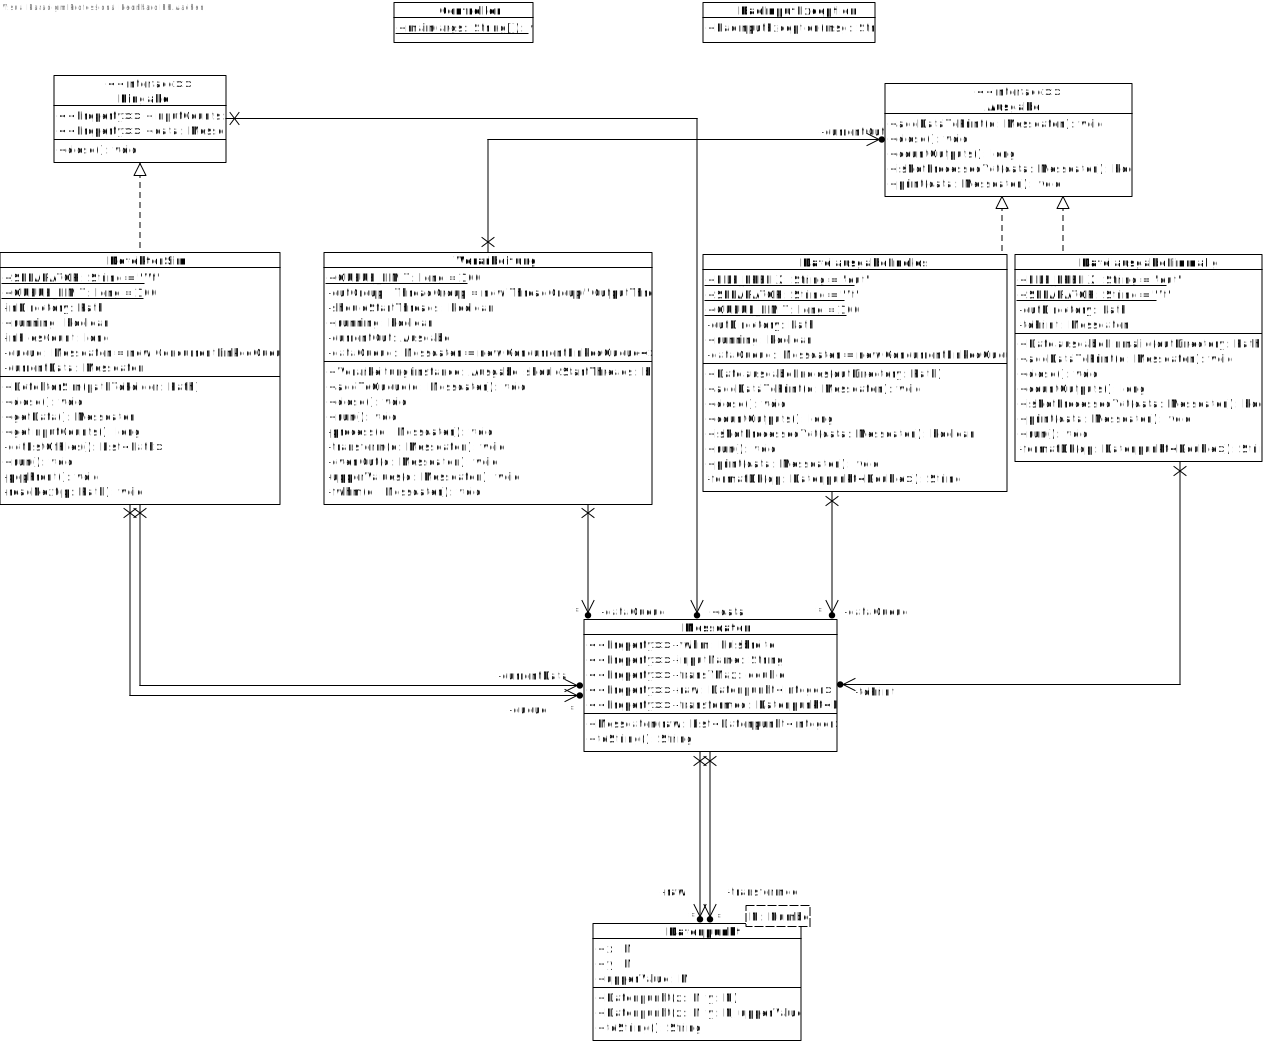
\includegraphics[width=0.9\paperwidth]{Class Diagram1}}
\end{center}

\fakesection{Struktogramme}\label{sec:structogram}
\fakesubsection{Controller.main()}\label{subsec:controller_main}
\begin{center}
    \makebox[\textwidth]{\includesvg[width=\textwidth]{Controller_main}}
\end{center}
\fakesubsection{Verarbeitung.transform()}\label{subsec:verarbeitung_transform}
\begin{center}
    \makebox[\textwidth]{\includesvg[width=\textwidth]{Verarbeitung_transform}}
\end{center}
\fakesubsection{Verarbeitung.evenOut()}\label{subsec:verarbeitung_evenOut}
\begin{center}
    \makebox[\textwidth]{\includesvg[width=\textwidth]{Verarbeitung_evenOut}}
\end{center}
\fakesubsection{Verarbeitung.upperValues()}\label{subsec:verarbeitung_uppverValues}
\begin{center}
    \makebox[\textwidth]{\includesvg[height=\textheight]{images/Verarbeitung_upperValues}}
\end{center}
\fakesubsection{Verarbeitung.fwhm()}\label{subsec:verarbeitung_fwhm}
\begin{center}
    \makebox[\textwidth]{\includesvg[width=\textwidth]{Verarbeitung_fwhm}}
\end{center}


\fakesection{Sequenzdiagramm}\label{sec:sequenzdiagramm}
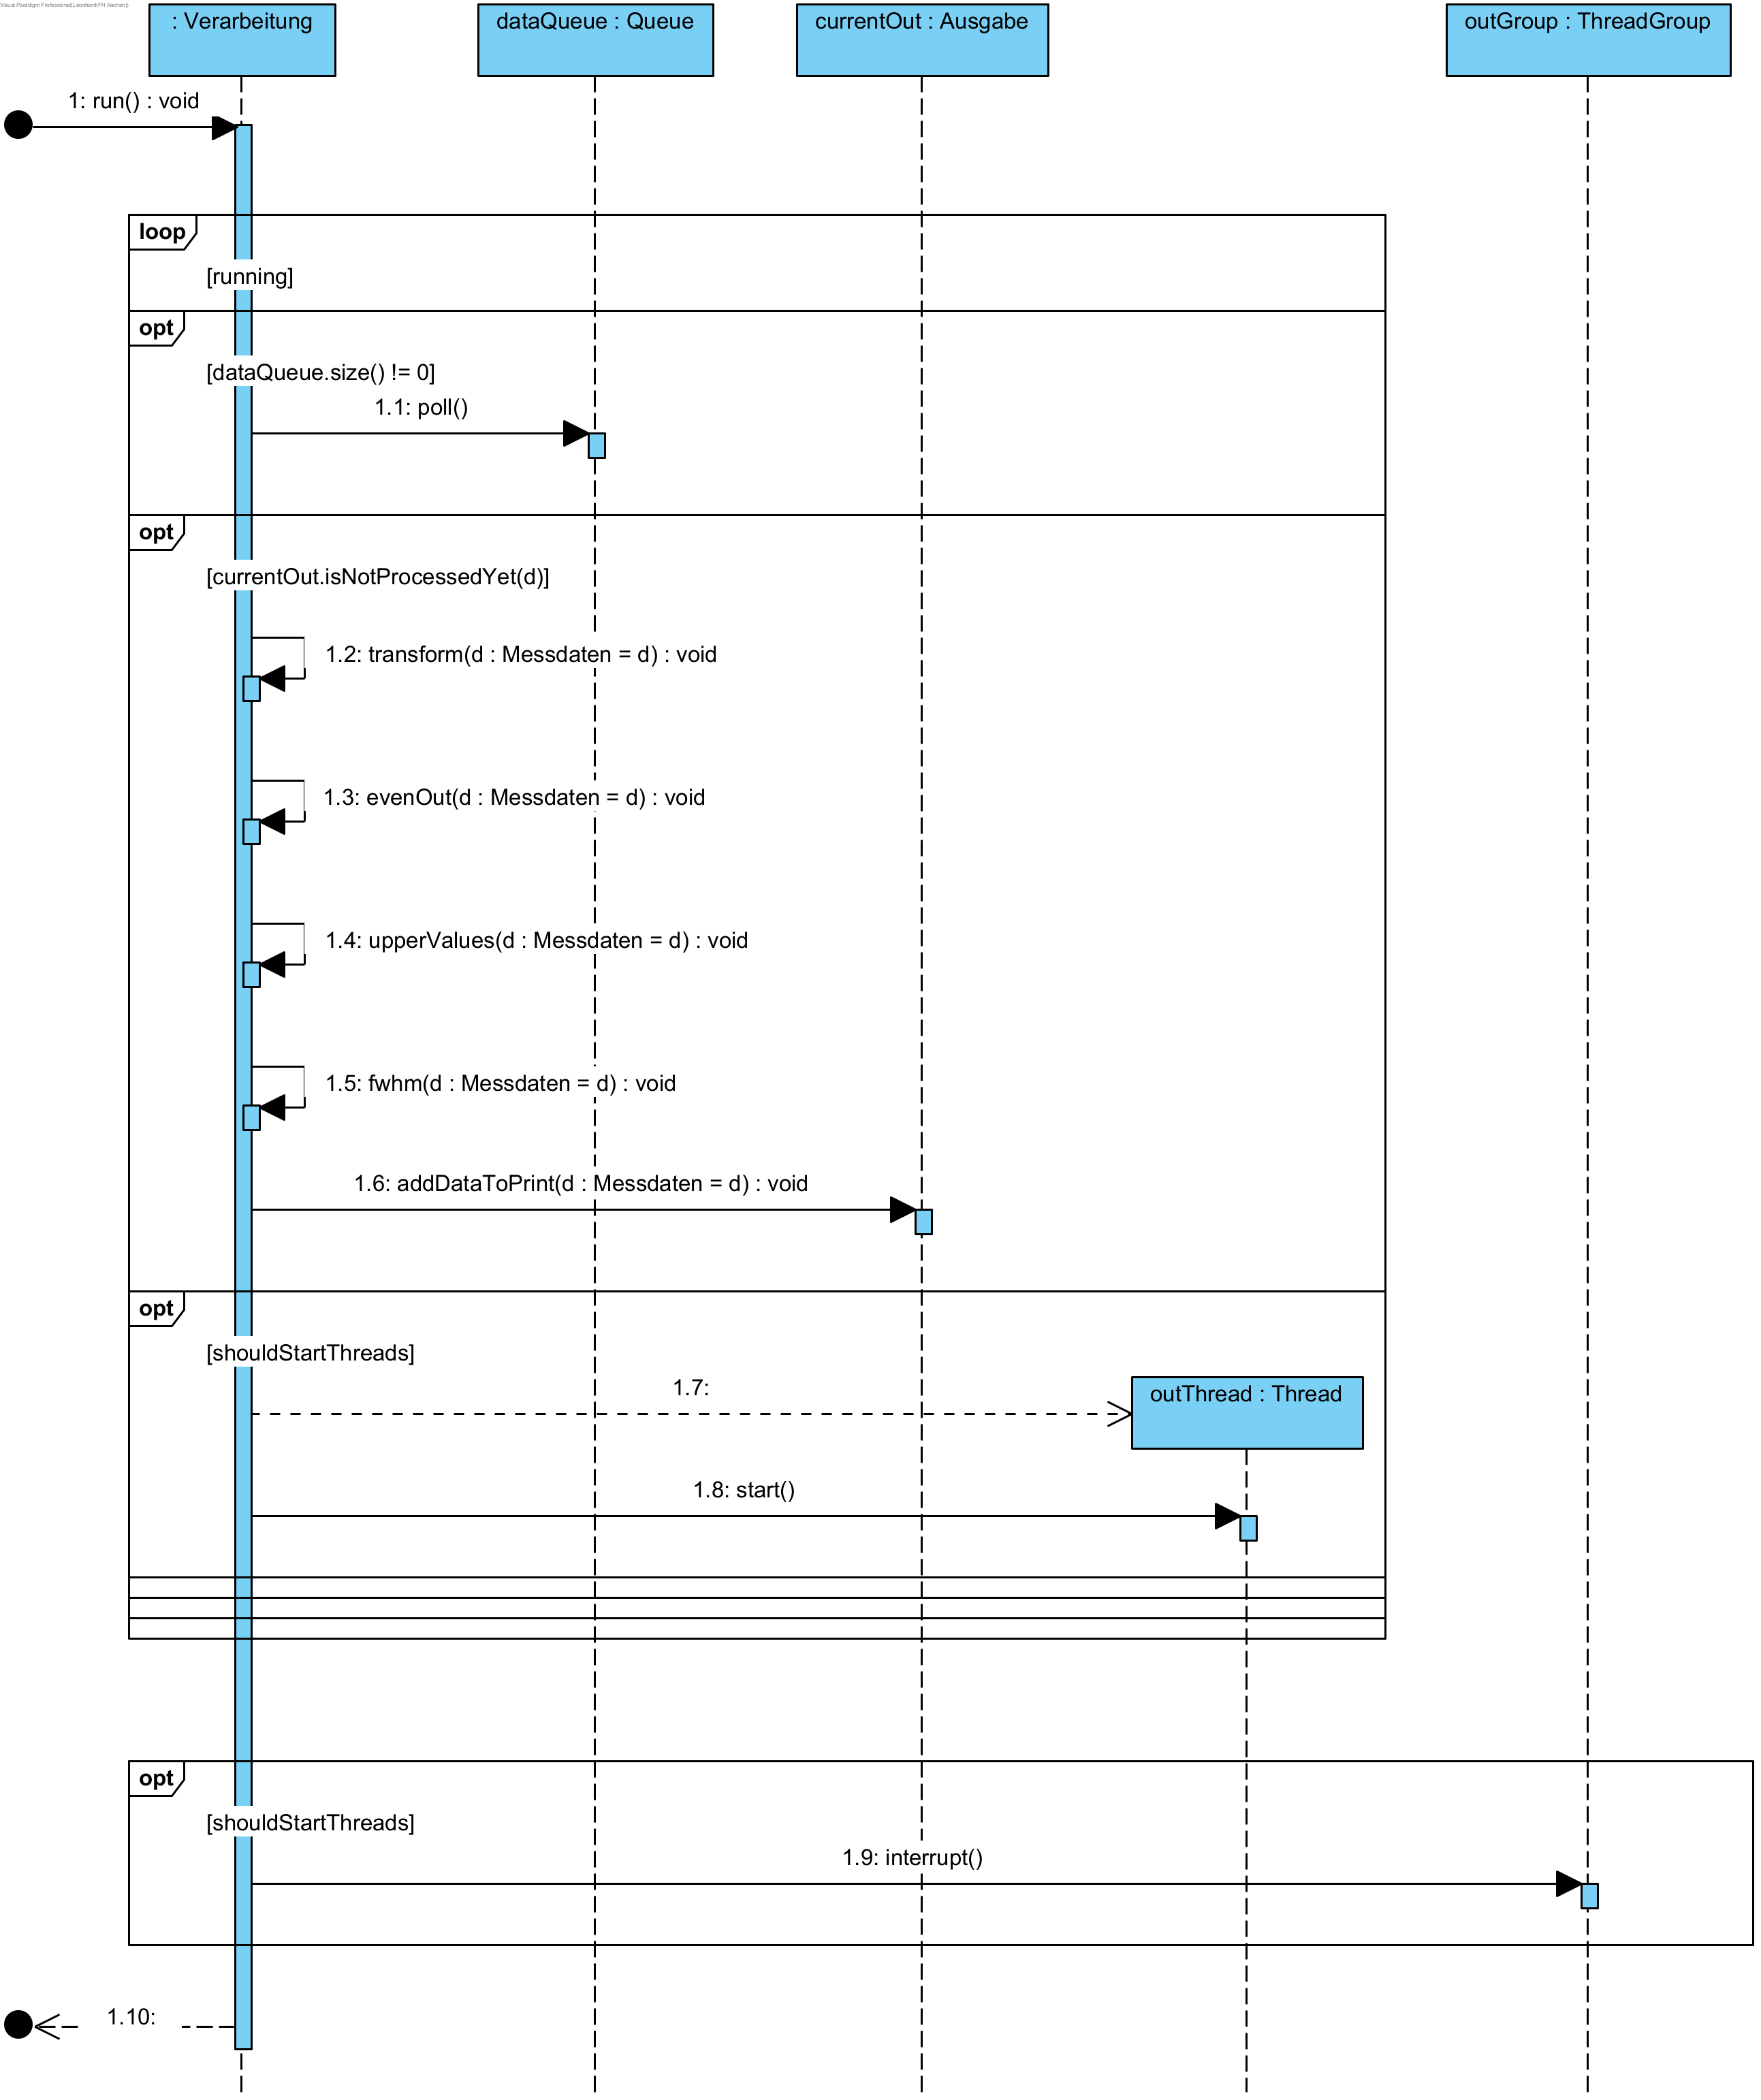
\includegraphics[width=\textwidth]{sequenz}


\section{Entwicklungsdokumentation}\label{sec:entwicklerdokumentation}
Die Dokumentation des Programms wurde in Javadoc vorgenommen und kann im Ordner javadoc eingesehen werden.
Hierzu kann die index.html aufgerufen werden.
%    \addtocontents{toc}{\protect\newpage}
    \chapter{Zusammenfassung und Ausblick}\label{ch:zusammenfassung-und-ausblick}


\section{Zusammenfassung}\label{sec:zusammenfassung}

\section{Ausblick}\label{sec:ausblick}


    % ============= Buchstabenteil ==============
    \renewcommand{\thechapter}{\Alph{chapter}}%
    \setcounter{chapter}{0}
    \chapter{Abweichung und Ergänzung}\label{ch:abweichung-und-ergaenzung}
-Thread -> Runnable
-Klassendiagramm
-Immer neuer Thread -> 3 (4) Threads insgesamt

    \chapter{Benutzeranleitung}\label{ch:benutzeranleitung}


\section{Vorbereiten des Systems}\label{sec:vorbereiten-des-systems}

\subsection{Systemvoraussetzungen}\label{subsec:systemvoraussetzungen}
Um sicherzustellen, dass das Programm lauffähig ist, sollte~\Betriebssystem~als Betriebssystem genutzt werden.
Es ist außerdem eine JRE oder JDK in der Version 17 oder höher vonnöten, um das Programm auszuführen.\\
Falls eine erneute Kompilierung des Programms gewünscht ist, empfiehlt es sich die JDK anstelle der JRE zu installieren.
Um diese JRE/JDK anschließend zu nutzen, muss das bin-Verzeichnis dieser in die PATH-Umgebungsvariable hinzugefügt werden.
\subsection{Installation}\label{subsec:installation}
Es ist keine Installation nötig, es reicht das~.zip-Verzeichnis zu entpacken.

\section{Programmaufruf}\label{sec:programmaufruf}
Nach dem Entpacken kann das Programm über den Befehl
\begin{center}
    \colorbox{gray!20}{
        \begin{minipage}{0.9\textwidth}
            java -jar GroPro-1.0.jar \grqq Testbeispiel\grqq~\grqq true\grqq
        \end{minipage}
    }
\end{center}
in der Eingabeaufforderung (CMD) oder beliebiger Bash ausgeführt werden.
Das erste Argument ist der Ordner, indem sich die~.txt-Dateien befinden.
Das zweite Argument ist ein boolean, über welchen die Ausgabevariante festgelegt werden kann.
Es ist optional und falls es true ist, wird die einmalige Ausgabe (siehe \nameref{subsec:ausgabe}) benutzt.
\section{Testen der Beispiele}\label{sec:testen-der-beispiele}
Das Ausführen der JAR erfolgt über die Datei \enquote{RunJar.cmd}.
In der Konsole wird nun das Programm für den Ordner \enquote{Testbeispiel} ausgeführt.
Alle Ausgaben befinden sich im Anschluss im Ordner \enquote{Testbeispiel/out}.

\section{Kompilieren}\label{sec:kompilieren}
Zum Erzeugen der~.jar-Datei sollte Maven genutzt werden.
Der Einfachheit halber muss das bin-Verzeichnis der Maveninstallation ebenfalls in der PATH-Umgebungsvariable aufgenommen werden.
Anschließend lässt sich das Programm kompilieren, indem der Befehl
\begin{center}
    \colorbox{gray!20}{
        \begin{minipage}{0.9\textwidth}
            mvn package
        \end{minipage}
    }
\end{center}
im Root-Verzeichnis des Quellcodes (das ist der Ordner, indem sich die \enquote{pom.xml} befindet) ausgeführt wird.
Eine JAR-Datei befindet sich dann im Ordner \enquote{target}.

\section{Visualisierung}\label{sec:visualisierung}
Das mitgelieferte Python-Programm \enquote{FileViewer.py} ist bereits so konfiguriert, dass es beim Ausführen über
\begin{center}
    \colorbox{gray!20}{
        \begin{minipage}{0.9\textwidth}
            python FileViewer.py
        \end{minipage}
    }
\end{center}
die Ausgabedateien mithilfe von matplot visualisiert.
    \include{chapters/C-Entwicklungsumgebung}
    \chapter{Verwendete Hilfsmittel}\label{ch:verwendete-hilfsmittel}

\begin{itemize}
    \item IntelliJ IDEA 2022.1 (Ultimate Edition)\\ Entwicklungsumgebung und Editor für Java und andere Programmiersprachen \\\url{https://www.jetbrains.com/de-de/idea/}
    \item Maven\\Build-Tool für Java\\\url{https://maven.apache.org}
    \item TexLive 2022\\Softwarepaket für \LaTeX\\\url{https://www.tug.org/texlive/}
    \item Structorizer\\Programm zur Erstellung von Nassi-Shneiderman-Diagrammen \\\url{https://structorizer.fisch.lu/}
    \item Visual Paradigm\\Programm zur Modellierung von Software-(Diagrammen) \\\url{https://www.visual-paradigm.com/}
    \item Git\\Versionsverwaltungssystem \\\url{https://git-scm.com/}
\end{itemize}
    \include{chapters/E-Erklaerung}
    \includepdf[scale=0.78, pages=2,pagecommand=\chapter{Aufgabenstellung}\label{ch:aufgabenstellung}, offset=0 -3cm]{images/Aufgabenstellung}
\includepdf[pages=3-]{images/Aufgabenstellung}
\end{document}